\documentclass[letterpaper,10pt,onecolumn]{article}
\usepackage[spanish]{babel}
\usepackage[latin1]{inputenc}
\usepackage{amsfonts}
\usepackage{amsthm}
\usepackage{amsmath}
\usepackage{mathrsfs}
\usepackage{empheq}
\usepackage{enumitem}
\usepackage[pdftex]{color,graphicx}
\usepackage{hyperref}
\usepackage{listings}
\usepackage{calligra}
\usepackage{algpseudocode} 
\DeclareMathAlphabet{\mathcalligra}{T1}{calligra}{m}{n}
\DeclareFontShape{T1}{calligra}{m}{n}{<->s*[2.2]callig15}{}
\newcommand{\scripty}[1]{\ensuremath{\mathcalligra{#1}}}
\lstloadlanguages{[5.2]Mathematica}
\setlength{\oddsidemargin}{0cm}
\setlength{\textwidth}{490pt}
\setlength{\textheight}{610pt}
\setlength{\topmargin}{-85pt}
\addtolength{\hoffset}{-0.3cm}
\addtolength{\textheight}{4cm}

\begin{document}
\thispagestyle{empty}
\begin{center}


\includegraphics[width=490pt]{figs/header.png}\\[0.5cm]

\textsc{\LARGE Bono - F\'isica I (FISI-1018) - Abril 14, 2016}\\[0.5cm]


\end{center}

\begin{enumerate}

\item (25 puntos)
Una bola peque\~na de masa $m$ se ubica sobre una bola m\'as
  grande de masa $M$. Las dos bolas se dejan caer desde una altura
  $h$. Calcule a que altura llega la bolita peque\~na despu\'es de la
  colisi\'on. Considere que todos los choques son el\'asticos y que
  $m$ es mucho menor que $M$.

\item 
Un carro de monta�a rusa se lanza desde una altura $h$. Encuentre
\begin{itemize}
\item (10 puntos) La velocidad que 
  tienen el carro en el punto $A$ (ver la figura).
\item (15 puntos) La altura m�nima de la cual se debe lanzar el carro para que llegue hasta el
punto $A$ (La respuesta debe estar dada en t�rminos de R).  
\end{itemize}

\item (25 puntos) Una bola de masa $m$ est� atada a un punto fijo por medio de una
  cuerda de longitud $L$. Un viento muy fuerte ejerce sobre la bola
  una fuerza constante, de magnitud $F$, de izquierda a derecha, como
  se muestra en la figura.  Si la bola estaba inicialmente en reposo,
  encuentre la altura m�xima que alcanza la bola $H_{max}$.


\item (25 puntos) Una bola de plastilina de masa $m$ es arrojada horizontalmente
  contra un bloque de madera de $M$ que se encuentra en reposo. La
  plastilina queda totalmente pegada al bloque de madera y el sistema
  queda en reposo luego de moverse una distancia $d$ con respecto a la
  posici�n inicial del bloque de madera. Si el coeficiente de fricci�n
  entre el bloque de madera y la superficie sobre la que se desliza es
  de $\mu$, �cu�l era la velocidad de la bola de plastilina justo
  antes de impactar al bloque de madera?  



\end{enumerate}

\begin{figure}[!h]
\begin{center}
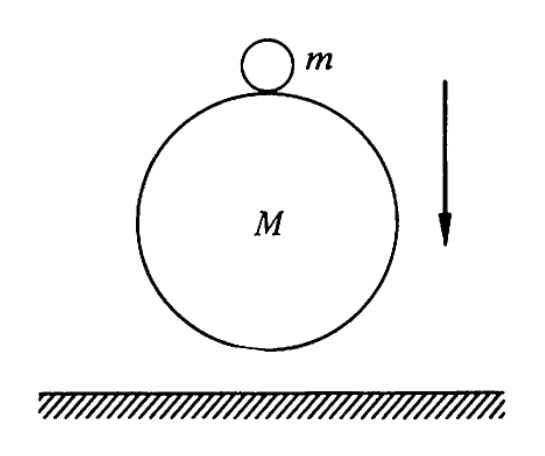
\includegraphics[scale=0.20]{pelotas.png}\\
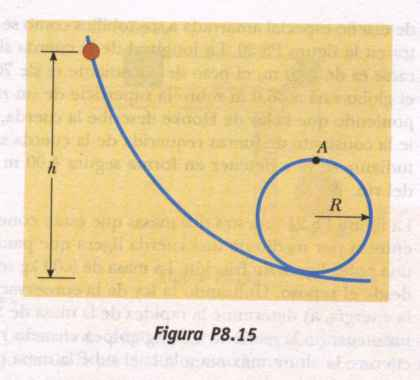
\includegraphics[scale=1.5]{montanarusa.jpg} 
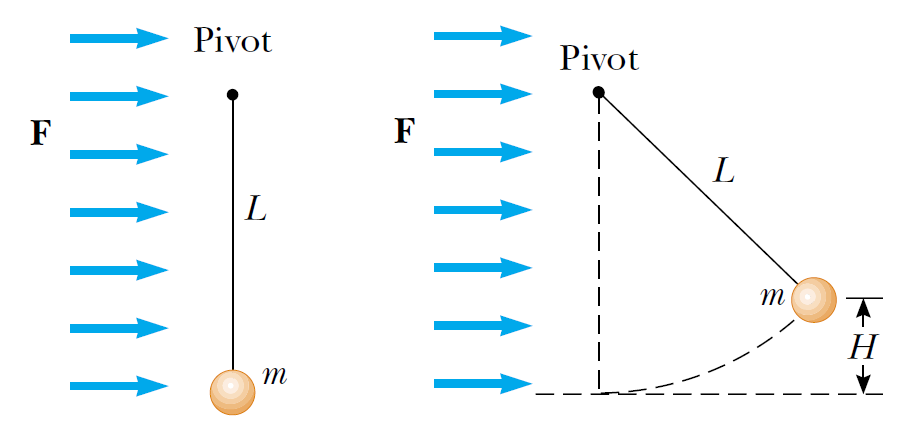
\includegraphics[scale=0.4]{bolaviento.PNG} 
\caption{Figuras para los ejercicios 1, 2 y 3 respectivamente.}
\end{center}
\end{figure}
{\small {\bf NOTA}: Todas las respuestas deben tener una justificaci\'on
f\'isica y matem\'atica adecuada. 100 puntos corresponden a una nota
de 5.0.}
\end{document}
